%
%===============>>  Сторожук Модуль 4 <<=============
%
\setmodule{4}
%
%===============>>  Занятие 1  <<===============
%
\begin{class}[number=1]
	\begin{listofex}
		\item Некоторая компания продает свою продукцию по цене p=400 руб. за единицу, переменные затраты на производство одной единицы продукции составляют \( v=200 \) руб., постоянные расходы предприятия \( f= 600000 \) руб. в месяц. Месячная операционная прибыль предприятия (в рублях) вычисляется по формуле \( \pi(q)=q(p-v)-f \). Определите месячный объeм производства \( q \) (единиц продукции), при котором месячная операционная прибыль предприятия будет равна \( 900 000 \) руб.
		\item Если достаточно быстро вращать ведeрко с водой на верeвке в вертикальной плоскости, то вода не будет выливаться. При вращении ведeрка сила давления воды на дно не остаeтся постоянной: она максимальна в нижней точке и минимальна в верхней. Вода не будет выливаться, если сила еe давления на дно будет положительной во всех точках траектории кроме верхней, где она может быть равной нулю. В верхней точке сила давления, выраженная в ньютонах, равна \( P=m \left( \dfrac{v^2}{L}-g \right) \), где \( m \) -- масса воды в килограммах, \( v \) скорость движения ведерка в м/с, \( L \) -- длина вервеки в метрах, \( g \) -- ускорение свободного падения (считайте \( g=10 \) м/с\( ^2 \)). С какой наименьшей скоростью надо вращать ведeрко, чтобы вода не выливалась, если длина верeвки равна \( 40 \) см? Ответ выразите в м/с.
		\item Камнеметательная машина выстреливает камни под некоторым острым углом к горизонту. Траектория полeта камня описывается формулой \( y=ax^2+bx \), где \( a=-\dfrac{1}{100} \) м\( ^{-1} \), \( b=1 \) -- постоянные параметры,\( x(M) \) -- смещение камня по горизонтали, \( y(M) \) -- высота камня над землeй. На каком наибольшем расстоянии (в метрах) от крепостной стены высотой \( 8 \) м нужно расположить машину, чтобы камни пролетали над стеной на высоте не менее \( 1 \) метра?
		\item Моторная лодка прошла против течения реки \( 112  \) км и вернулась в пункт отправления, затратив на обратный путь на \( 6 \) часов меньше. Найдите скорость течения, если скорость лодки в неподвижной воде равна \( 11 \) км/ч. Ответ дайте в км/ч.
		\item Теплоход проходит по течению реки до пункта назначения \( 200 \) км и после стоянки возвращается в пункт отправления. Найдите скорость течения, если скорость теплохода в неподвижной воде равна \( 15 \) км/ч, стоянка длится \( 10 \) часов, а в пункт отправления теплоход возвращается через \( 40 \) часов после отплытия из него. Ответ дайте в км/ч.
		\item Пристани \( A \) и \( B \) расположены на озере, расстояние между ними 390 км. Баржа отправилась с постоянной скоростью из \( A \) в \( B \). На следующий день после прибытия она отправилась обратно со скоростью на \( 3 \) км/ч больше прежней, сделав по пути остановку на \( 9 \) часов. В результате она затратила на обратный путь столько же времени, сколько на путь из \( A \) в \( B \). Найдите скорость баржи на пути из \( A \) в \( B \). Ответ дайте в км/ч.
		\item Из пункта \( A \) в пункт \( B \), расстояние между которыми \( 75 \) км, одновременно выехали автомобилист и велосипедист. Известно, что за час автомобилист проезжает на \( 40 \) км больше, чем велосипедист. Определите скорость велосипедиста, если известно, что он прибыл в пункт \( B \) на \( 6 \) часов позже автомобилиста. Ответ дайте в км/ч.
		\item Велосипедист выехал с постоянной скоростью из города \( A \) в город \( B \), расстояние между которыми равно \( 70 \) км. На следующий день он отправился обратно в \( A \) со скоростью на \( 3 \) км/ч больше прежней. По дороге он сделал остановку на \( 3 \) часа. В результате велосипедист затратил на обратный путь столько же времени, сколько на путь из \( A \) в \( B \). Найдите скорость велосипедиста на пути из \( B \) в \( A \). Ответ дайте в км/ч.
	\end{listofex}
\end{class}
%
%===============>>  Занятие 2  <<===============
%
\begin{class}[number=2]
	\begin{listofex}
		\item Два тела массой \( m=2 \) кг каждое, движутся с одинаковой скоростью  \( v =10  \)м/с под углом \( 2\alpha \)  друг к другу. Энергия (в джоулях), выделяющаяся при их абсолютно неупругом соударении определяется выражением \( Q=mv^2\sin^2\alpha \). Под каким наименьшим углом \( 2\alpha \) (в градусах) должны двигаться тела, чтобы в результате соударения выделилось не менее \( 50 \) джоулей?
		\item Моторная лодка прошла против течения реки \( 255 \) км и вернулась в пункт отправления, затратив на обратный путь на \( 2 \) часа меньше. Найдите скорость лодки в неподвижной воде, если скорость течения равна \( 1 \) км/ч. Ответ дайте в км/ч.
		\item Теплоход проходит по течению реки до пункта назначения \( 255 \) км и после стоянки возвращается в пункт отправления. Найдите скорость теплохода в неподвижной воде, если скорость течения равна \( 1 \) км/ч, стоянка длится \( 2 \) часа, а в пункт отправления теплоход возвращается через \( 34 \) часа после отплытия из него. Ответ дайте в км/ч.
		\item Баржа в \( 10:00 \) вышла из пункта \( A \) в пункт \( B \), расположенный в \( 15 \) км от \( A \). Пробыв в пункте B \( 1 \) час \( 20 \) минут, баржа отправилась назад и вернулась в пункт \( A \) в \( 16:00 \) того же дня. Определите (в км/час) скорость течения реки, если известно, что собственная скорость баржи равна \( 7 \) км/ч.
		\item Моторная лодка в \( 10:00 \) вышла из пункта \( А \) в пункт \( В \), расположенный в \( 30 \) км от \( А \). Пробыв в пункте \( В \) \( 2 \) часа \( 30 \) минут, лодка отправилась назад и вернулась в пункт \( А \) в \( 18:00 \) того же дня. Определите (в км/ч) собственную скорость лодки, если известно, что скорость течения реки \( 1 \) км/ч.
		\item Первые \( 190 \) км автомобиль ехал со скоростью \( 50 \) км/ч, следующие \( 180 \) км -- со скоростью \( 90 \) км/ч, а затем \( 170 \) км -- со скоростью \( 100 \) км/ч. Найдите среднюю скорость автомобиля на протяжении всего пути. Ответ дайте в км/ч.
		\item Первые два часа автомобиль ехал со скоростью \( 50 \) км/ч, следующий час -- со скоростью \( 100 \) км/ч, а затем два часа -- со скоростью \( 75 \) км/ч. Найдите среднюю скорость автомобиля на протяжении всего пути. Ответ дайте в км/ч.
		\item Из городов \( A \) и \( B \), расстояние между которыми равно \( 330 \) км, навстречу друг другу одновременно выехали два автомобиля и встретились через \( 3 \) часа на расстоянии \( 180 \) км от города \( B \). Найдите скорость автомобиля, выехавшего из города \( A \). Ответ дайте в км/ч.
		\item Два велосипедиста одновременно отправились в \( 88 \)-километровый пробег. Первый ехал со скоростью, на \( 3 \) км/ч большей, чем скорость второго, и прибыл к финишу на \( 3 \) часа раньше второго. Найти скорость велосипедиста, пришедшего к финишу вторым. Ответ дайте в км/ч.
	\end{listofex}
\end{class}
%
%===============>>  Домашняя работа 1  <<===============
%
\begin{homework}[number=1]
	\begin{listofex}
		\item Велосипедист выехал с постоянной скоростью из города \( A \) в город \( B \), расстояние между которыми равно \( 154 \) км. На следующий день он отправился обратно со скоростью на \( 3 \) км/ч больше прежней. По дороге он сделал остановку на \( 3 \) часа. В результате он затратил на обратный путь столько же времени, сколько на путь из \( A \) в \( B \). Найдите скорость велосипедиста на пути из \( A \) в \( B \). Ответ дайте в км/ч.
		\item Из городов \( A \) и \( B \), расстояние между которыми равно \( 300 \) км, навстречу друг другу одновременно выехали два автомобиля и встретились через \( 2 \) часа на расстоянии \( 180 \) км от города \( B \). Найдите скорость автомобиля, выехавшего из города \( A \). Ответ дайте в км/ч.
		\item От пристани \( A \) к пристани \( B \), расстояние между которыми равно \( 224 \) км, отправился с постоянной скоростью первый теплоход, а через \( 2 \) часа после этого следом за ним со скоростью на \( 2 \) км/ч большей отправился второй. Найдите скорость второго теплохода, если в пункт \( B \) он прибыл одновременно с первым. Ответ дайте в км/ч.
		\item Ёмкость высоковольтного конденсатора в телевизоре \( C=2\cdot10^{-6} \) Ф. Параллельно с конденсатором подключeн резистор с сопротивлением \( R=5\cdot10^6 \) Ом. Во время работы телевизора напряжение на конденсаторе \(  U_0 = 16 \) кВ. После выключения телевизора напряжение на конденсаторе убывает до значения \( U \) (кВ) за время, определяемое выражением \( t=\alpha RC\log_2\dfrac{U}{U_0} \) (с), где \( \alpha=0,7 \) -- постоянная. Определите напряжение на конденсаторе, если после выключения телевизора прошло \( 21 \) с. Ответ дайте в киловольтах.
		\item \exercise{1244}
	\end{listofex}
\end{homework}
%
%===============>>  Занятие 3  <<===============
%
\begin{class}[number=3]
	\begin{listofex}
		\item \exercise{1234}
		\item \exercise{1242}
		\item \exercise{1260}
		\item \exercise{1264}
		\item Два мотоциклиста стартуют одновременно в одном направлении из двух диаметрально противоположных точек круговой трассы, длина которой равна \( 14 \) км. Через сколько минут мотоциклисты поравняются в первый раз, если скорость одного из них на \( 21 \) км/ч больше скорости другого?
		\item Два гонщика участвуют в гонках. Им предстоит проехать \( 60 \) кругов по кольцевой трассе протяжённостью \( 3 \) км. Оба гонщика стартовали одновременно, а на финиш первый пришёл раньше второго на \( 10 \) минут. Чему равнялась средняя скорость второго гонщика, если известно, что первый гонщик в первый раз обогнал второго на круг через \( 15 \) минут? Ответ дайте в км/ч.
		\item Часы со стрелками показывают \( 8 \) часов ровно. Через сколько минут минутная стрелка в четвертый раз поравняется с часовой?
		\item Из пункта \( A \) круговой трассы выехал велосипедист. Через \( 30 \) минут он еще не вернулся в пункт \( A \) и из пункта \( A \) следом за ним отправился мотоциклист. Через \( 10 \) минут после отправления он догнал велосипедиста в первый раз, а еще через \( 30 \) минут после этого догнал его во второй раз. Найдите скорость мотоциклиста, если длина трассы равна \( 30 \) км. Ответ дайте в км/ч.
		\item Рабочие прокладывают тоннель длиной \( 500 \) метров, ежедневно увеличивая норму прокладки на одно и то же число метров. Известно, что за первый день рабочие проложили \( 3 \) метра тоннеля. Определите, сколько метров тоннеля проложили рабочие в последний день, если вся работа была выполнена за \( 10 \) дней.
		\item Васе надо решить \( 434 \) задачи. Ежедневно он решает на одно и то же количество задач больше по сравнению с предыдущим днем. Известно, что за первый день Вася решил \( 5 \) задач. Определите, сколько задач решил Вася в последний день, если со всеми задачами он справился за \( 14 \) дней.
		\item Компания «Альфа» начала инвестировать средства в перспективную отрасль в \( 2001 \) году, имея капитал в размере \( 5000 \) долларов. Каждый год, начиная с \( 2002 \) года, она получала прибыль, которая составляла \( 200\% \) от капитала предыдущего года. А компания «Бета» начала инвестировать средства в другую отрасль в \( 2003 \) году, имея капитал в размере \( 10 000 \) долларов, и, начиная с \( 2004 \) года, ежегодно получала прибыль, составляющую \( 400\% \) от капитала предыдущего года. На сколько долларов капитал одной из компаний был больше капитала другой к концу \( 2006 \) года, если прибыль из оборота не изымалась?
		\item \exercise{1249}
	\end{listofex}
\end{class}
%
%===============>>  Занятие 4  <<===============
%
%\begin{class}[number=4]
%	\begin{listofex}
%		\item Пусто
%	\end{listofex}
%\end{class}
%
%===============>>  Домашняя работа 2  <<===============
%
\begin{homework}[number=2]
	\begin{listofex}
		\item Из одной точки круговой трассы, длина которой равна \( 14 \) км, одновременно в одном направлении стартовали два автомобиля. Скорость первого автомобиля равна \( 80 \) км/ч, и через \( 40 \) минут после старта он опережал второй автомобиль на один круг. Найдите скорость второго автомобиля. Ответ дайте в км/ч.
		\item Бригада маляров красит забор длиной \( 240 \) метров, ежедневно увеличивая норму покраски на одно и то же число метров. Известно, что за первый и последний день в сумме бригада покрасила \( 60 \) метров забора. Определите, сколько дней бригада маляров красила весь забор.
		\item Компания "Альфа" начала инвестировать средства в перспективную отрасль в \( 2001 \) году, имея капитал в размере \( 3000 \) долларов. Каждый год, начиная с \( 2002 \) года, она получала прибыль, которая составляла \( 100\% \) от капитала предыдущего года. А компания "Бета" начала инвестировать средства в другую отрасль в \( 2004 \) году, имея капитал в размере \( 4500 \) долларов, и, начиная с \( 2005 \) года, ежегодно получала прибыль, составляющую \( 300\% \) от капитала предыдущего года. На сколько долларов капитал одной из компаний был больше капитала другой к концу \( 2008 \) года, если прибыль из оборота не изымалась?
		\item При адиабатическом процессе для идеального газа выполняется закон \( pV^k=10^5 \)  Па\( \cdot \)на м\( ^5 \), где \( p \) -- давление газа в паскалях, \( V \) -- объeм газа в кубических метрах, \( k=\dfrac{5}{3} \).  Найдите, какой объём \( V \) (в куб. м) будет занимать газ при давлении \( p \), равном \( 3,2\cdot10^6 \) Па.
		\item \exercise{1263}
	\end{listofex}
\end{homework}
%
%===============>>  Занятие 5  <<===============
%
\begin{class}[number=6]
	\begin{listofex}
		\item Клиент А. сделал вклад в банке в размере \( 7700  \) рублей. Проценты по вкладу начисляются раз в год и прибавляются к текущей сумме вклада. Ровно через год на тех же условиях такой же вклад в том же банке сделал клиент Б. Еще ровно через год клиенты А. и Б. закрыли вклады и забрали все накопившиеся деньги. При этом клиент А. получил на \( 847  \) рублей больше клиента Б. Какой процент годовых начислял банк по этим вкладам?
		\item Смешали некоторое количество \( 15\% \)-го раствора некоторого вещества с таким же количеством \( 19\% \)-го раствора этого вещества. Сколько процентов составляет концентрация получившегося раствора?
		\item Смешав \( 30 \)-процентный и \( 60 \)-процентный растворы кислоты и добавив \( 10 \) кг чистой воды, получили \( 36 \)-процентный раствор кислоты. Если бы вместо \( 10 \) кг воды добавили \( 10 \) кг \( 50 \)-процентного раствора той же кислоты, то получили бы \( 41 \)-процентный раствор кислоты. Сколько килограммов \( 30 \)-процентного раствора использовали для получения смеси?
		\item Первая труба наполняет резервуар на \( 6 \) минут дольше, чем вторая. Обе трубы наполняют этот же резервуар за \( 4  \) минуты. За сколько минут наполняет этот резервуар одна вторая труба?
		\item Первый насос наполняет бак за \( 20  \) минут, второй --- за \( 30 \) минут, а третий --- за \( 1  \) час. За сколько минут наполнят бак три насоса, работая одновременно?
		\item Две трубы наполняют бассейн за \( 3 \) часа \( 36 \) минут, а одна первая труба наполняет бассейн за \( 6 \) часов. За сколько часов наполняет бассейн одна вторая труба?
		\item Заказ на \( 110 \) деталей первый рабочий выполняет на \( 1 \) час быстрее, чем второй. Сколько деталей за час изготавливает второй рабочий, если известно, что первый за час изготавливает на \( 1 \) деталь больше?
		\item Заказ на \( 156 \) деталей первый рабочий выполняет на \( 1 \) час быстрее, чем второй. Сколько деталей за час изготавливает первый рабочий, если известно, что он за час изготавливает на \( 1 \) деталь больше второго?
		\item Каждый из двух рабочих одинаковой квалификации может выполнить заказ за \( 15 \) часов. Через \( 3 \) часа после того, как один из них приступил к выполнению заказа, к нему присоединился второй рабочий, и работу над заказом они довели до конца уже вместе. Сколько часов потребовалось на выполнение всего заказа?
		\item На изготовление \( 99 \) деталей первый рабочий тратит на \( 2 \) часа меньше, чем второй рабочий на изготовление \( 110 \) таких же деталей. Известно, что первый рабочий за час делает на \( 1 \) деталь больше, чем второй. Сколько деталей в час делает второй рабочий?
		\item Двое рабочих, работая вместе, могут выполнить работу за \( 12 \) дней. За сколько дней, работая отдельно, выполнит эту работу первый рабочий, если он за два дня выполняет такую же часть работы, какую второй --- за три дня?
	\end{listofex}
\end{class}
%
%===============>>  Занятие 6  <<===============
%
\begin{class}[number=6]
	\begin{listofex}
		\item \mexercise{_78}
		\item Найдите значение выражения:
		\begin{enumcols}[itemcolumns=3]
			\item \( (\log_216)\cdot(\log_636) \)
			\item \( 7\cdot5^{\log_54} \)
			\item \( 36^{\log_65} \)
			\item \( \log_{0,25}2 \)
			\item \( \log_48 \)
			\item \( \log_560-\log_512 \)
			\item \( \log_50,2+\log_{0,5}4 \)
			\item \( \log_{0,3}10-\log_{0,3}3 \)
			\item \( \dfrac{\log_325}{\log_35} \)
			\item \( \dfrac{\log_713}{\log_{49}13} \)
			\item \( \log_59\cdot\log_325 \)
			\item \( \dfrac{9^{\log_550}}{9^{\log_52}} \)
			\item \( 6\log_4\sqrt[3]{7} \)
			\item \( \log_{\sqrt[6]{13}}13 \)
			\item \( \dfrac{\log_318}{2+\log_32} \)
			\item \( \dfrac{\log_35}{\log_37}+\log_70,2 \)
			\item \( \log_{0,8}3\log_31,25 \)
			\item \( 5^{\log_{25}49} \)
			\item \( \log^2_{\sqrt{7}}49 \)
			\item \( 5^{3+\log_52} \)
			\item \( 8^{2+\log_83} \)
			\item \( 64^{\log_8\sqrt{3}} \)
			\item \( \log_4\log_525 \)
			\item \( \dfrac{24}{3^{\log_32}} \)
			\item \( \log_{\dfrac{1}{13}}\sqrt{13} \)
			\item \( \log_38,1+\log_310 \)
			\item \( \dfrac{\log_6\sqrt{13}}{\log_613} \)
			\item \( \left( 3^{\log_23} \right)^{\log_32}\)
			\item \( \log_57\cdot\log_725 \)
			\item \( \dfrac{\log_212,8-\log_20,8}{5^{\log_{25}16}} \)
			\item \( \dfrac{\log_23,2-\log_20,2}{3^{\log_925}} \)
			\item \( 3^{\log_37}+49^{\log_7{\sqrt{13}}} \)
		\end{enumcols}
		\item Улитка ползет от одного дерева до другого. Каждый день она проползает на одно и то же расстояние больше, чем в предыдущий день. Известно, что за первый и последний дни улитка проползла в общей сложности \( 8 \) метров. Определите, сколько дней улитка потратила на весь путь, если расстояние между деревьями равно \( 28 \) метрам.
		\item Бизнесмен Бубликов получил в \( 2000 \) году прибыль в размере \( 5000  \) рублей. Каждый следующий год его прибыль увеличивалась на \( 300\% \) по сравнению с предыдущим годом. Сколько рублей заработал Бубликов за \( 2003 \) год?
		\item Два гонщика участвуют в гонках. Им предстоит проехать 60 кругов по кольцевой трассе протяжённостью \( 3 \) км. Оба гонщика стартовали одновременно, а на финиш первый пришёл раньше второго на 10 минут. Чему равнялась средняя скорость второго гонщика, если известно, что первый гонщик в первый раз обогнал второго на круг через \( 15 \) минут? Ответ дайте в км/ч.
		\item Теплоход, скорость которого в неподвижной воде равна \( 20 \) км/ч, проходит по течению реки и после стоянки возвращается в исходный пункт. Скорость течения равна \( 4 \) км/ч, стоянка длится \( 2 \) часа, а в исходный пункт теплоход возвращается через \( 42 \) часа после отплытия из него. Сколько километров прошел теплоход за весь рейс?
	\end{listofex}
\end{class}
%
%===============>>  Домашняя работа 3  <<===============
%
%\begin{homework}[number=3]
%	\begin{listofex}
%		\item Пусто
%	\end{listofex}
%\end{homework}
%
%===============>>  Занятие 7  <<===============
%
\begin{class}[number=7]
	\begin{listofex}
			\item Вычислить:
	\begin{enumcols}[itemcolumns=3]
		\item \exercise{562}
		\item \exercise{564}
		\item \exercise{569}
		\item \exercise{571}
		\item \exercise{579}
	\end{enumcols}
	\item Вычислить:
	\begin{enumcols}[itemcolumns=3]
		\item \exercise{1577}
		\item \exercise{1578}
		\item \exercise{1579}
	\end{enumcols}
	\item Вычислить:
	\begin{enumcols}[itemcolumns=3]
		\item \exercise{1572}
		\item \exercise{1565}
		\item \exercise{1566}
		\item \exercise{1573}
		\item \exercise{1567}
		\item \exercise{1575}
		\item \exercise{1594}
	\end{enumcols}
	\item Вычислить:
	\begin{enumcols}[itemcolumns=2]
		\item \exercise{1569}
		\item \exercise{1570}
		\item \exercise{1571}
		\item \exercise{1574}
	\end{enumcols}
		\item Решите уравнение:
\begin{enumcols}[itemcolumns=2]
	\item \( \log_2(4-x)=7 \)
	\item \( \log_5(5-x)=\log_53 \)
	\item \( \log_4(x+3)=\log_4(4x-15) \)
	\item \( \log_{\frac{1}{7}}(7-x)=-2 \)
	\item \( \log_5(5-x)=2\log_53 \)
	\item \( \log_5(x^2+2x)=\log_5(x^2+10) \)
	\item \( \log_x32=5 \)	
	\item \( \log_{x-5}49=2 \)
	\item \( \log_82^{8x-4}=4 \)
	\item \( 2^{\log_8(5x-3)}=4 \)
	\end{enumcols}
	\item \exercise{1261}
	\item Водолазный колокол, содержащий в начальный момент времени  \( v = 3 \) моль воздуха объeмом \( V_1=8 \) л, медленно опускают на дно водоeма. При этом происходит изотермическое сжатие воздуха до конечного объeма \( V_2 \). Работа, совершаемая водой при сжатии воздуха, определяется выражением \( A=\alpha vT\log_2\dfrac{V_1}{V_2} \) (Дж), где \(  \alpha=5,75 \) --- постоянная, а \( T = 300 \)К --- температура воздуха. Какой объeм \( V_2 \) (в литрах) станет занимать воздух, если при сжатии газа была совершена работа в \( 10 350 \) Дж?	
	\end{listofex}
\end{class}
%===============>>  Проверочная работа  <<===============
%
\begin{class}[number=8]
	\begin{listofex}
		\item
		\begin{minipage}[t]{0.67\textwidth}
			На рисунке изображен график функции \( f(x)=kx+b \). Найдите \( f(-9) \).
		\end{minipage}
		\begin{minipage}[c]{0.2\textwidth}
			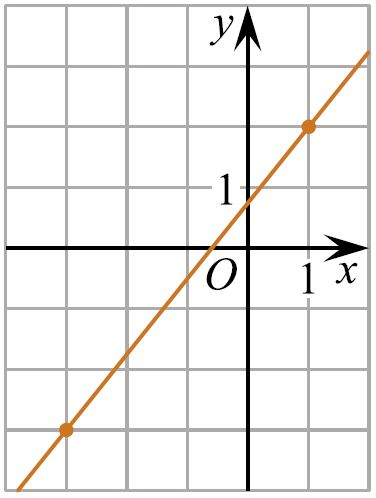
\includegraphics[align=t, width=0.8\textwidth]{pics/G112M3C2-1}
		\end{minipage}
		\item
		\begin{minipage}[t]{0.67\textwidth}
			На рисунке изображены графики двух линейных функций. Найдите абсциссу точки пересечения графиков.
		\end{minipage}
		\begin{minipage}[c]{0.2\textwidth}
			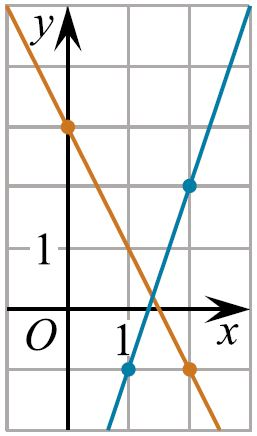
\includegraphics[align=t, width=0.8\textwidth]{pics/G112M3C2-2}
		\end{minipage}
		\item
		\begin{minipage}[t]{0.57\textwidth}
			На рисунке изображен график функции \( f(x)=\dfrac{x^2}{a}+bx+c \). Найдите \( f(3,5) \).
		\end{minipage}
		\begin{minipage}[c]{0.3\textwidth}
			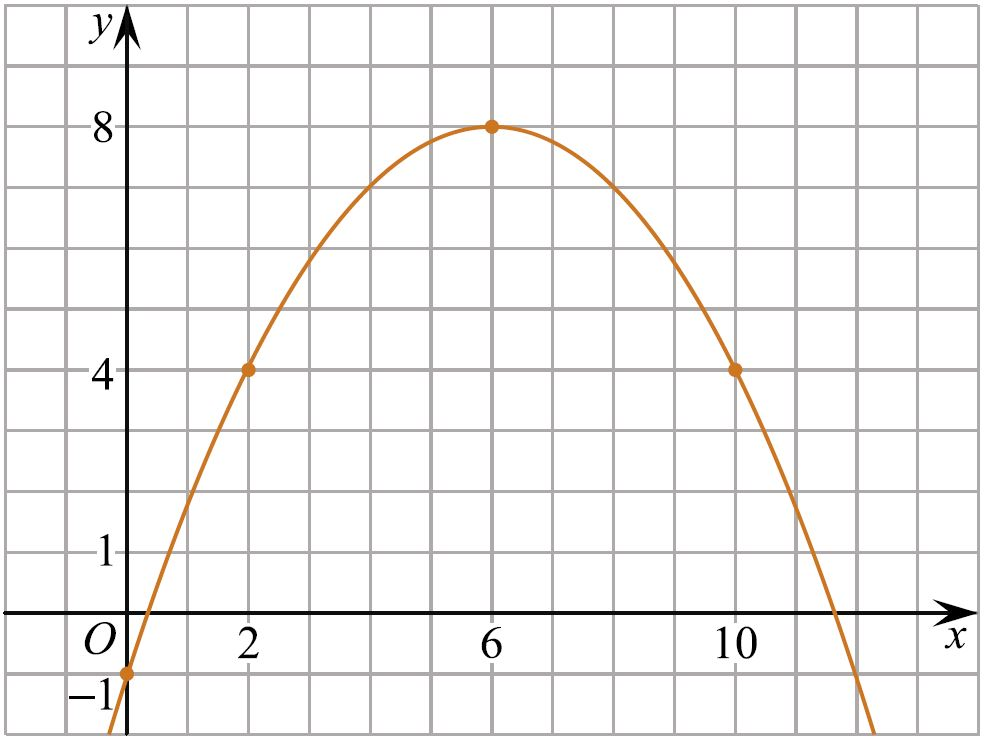
\includegraphics[align=t, width=\textwidth]{pics/G112M3C2-3}
		\end{minipage}
		\item
		\begin{minipage}[t]{0.57\textwidth}
			На рисунке изображен график функции \( f(x)=\dfrac{x^2}{a}+bx+c \). Найдите \( f(4) \).
		\end{minipage}
		\begin{minipage}[c]{0.3\textwidth}
			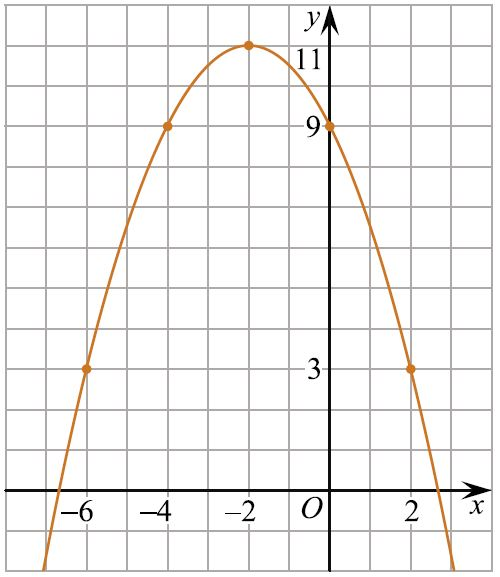
\includegraphics[align=t, width=\textwidth]{pics/G112M3C2-4}
		\end{minipage}
		\item
		\begin{minipage}[t]{0.57\textwidth}
			На рисунке изображены графики функций \( f(x)=2x^2+11x+11 \) и \( y=ax^2+bx+c \), которые пересекаются в точках \( A \) и \( B \). Найдите абсциссу точки \( B \).
		\end{minipage}
		\begin{minipage}[c]{0.3\textwidth}
			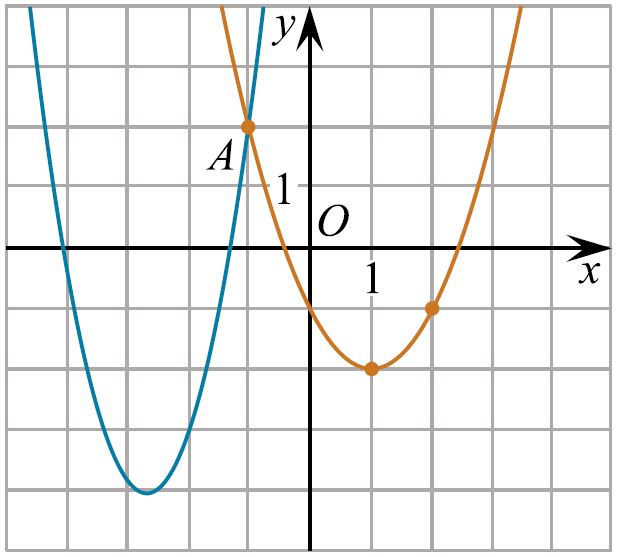
\includegraphics[align=t, width=\textwidth]{pics/G112M3C2-6}
		\end{minipage}
		\item Велосипедист выехал с постоянной скоростью из города \( A \) в город \( B \), расстояние между
		которыми равно \( 70 \) км. На следующий день он отправился обратно в \( A \) со скоростью на \( 3 \) км/ч больше прежней. По дороге он сделал остановку на \( 3 \) часа. В результате велосипедист затратил на обратный путь столько же времени, сколько на путь из \( A \) в \( B \). Найдите скорость велосипедиста на пути из \( B \) в \( A \). Ответ дайте в км/ч.
		\item В сосуд, содержащий \( 5 \) литров \( 12 \)--процентного водного раствора некоторого вещества,
		добавили \( 7 \) литров воды. Сколько процентов составляет концентрация получившегося раствора?
	\end{listofex}
\end{class}